\renewcommand{\thesection}{\arabic{section}.\arabic{section}}
% \renewcommand{\thesection}{\Alph{section}.\arabic{section}}
\setcounter{section}{0}


\begin{appendices}
\chapter{Vector Calculus}
\section{Differentiate}

\subsection{Differentiation Rules}

\begin{itemize}
	\item Product rule: 
		$$(f(x)g(x))' = f'(x)g(x)+f(x)g'(x)$$
	\item Quotient rule: 
		$$\left(\frac{f(x)}{g(x)}\right)' = \frac{f'(x)g(x)+f(x)g'(x)}{(g(x))^2}$$
	\item Sum rule: 
		$$(f(x)+g(x))' = f'(x)+g'(x)$$
	\item Chain rule:
		$$(g(f(x)))' = g'(f(x))f'(x)$$
\end{itemize}

The generalization of the derivative to functions of several variables is the \textit{gradient}. We find the gradient of the function $f$ with respect to $x$ by varying one variable at a time and keeping the others constant. \textbf{The gradient is then the collection of these partial derivatives}.

For example, partial derivatives using the chain rule of $f(x,y) = (x+2y^3)^2$ is given by
\[ \frac{\partial f(x, y)}{\partial x} = 2(x + 2y^3) \frac{\partial}{\partial x}(x + 2y^3) = 2(x + 2y^3) \]

\paragraph{Basic rules of Partial Differentiation:} 
\begin{itemize}
	\item Product rule:
	\[ \frac{\partial}{\partial \rvx} \big[f(\rvx)g(\rvx)\big] = \frac{\partial f}{\partial \rvx} g(\rvx) + f(\rvx) \frac{\partial g}{\partial \rvx} \]
	\item Sum rule:
	\[ \frac{\partial}{\partial \rvx} \big[f(\rvx) + g(\rvx)\big] = \frac{\partial f}{\partial \rvx} + \frac{\partial g}{\partial \rvx} \]
	\item Chain rule:
	\[ \frac{\partial}{\partial \rvx} (g \circ f)(\rvx) = \frac{\partial}{\partial \rvx} \big[g(f(\rvx))\big] = \frac{\partial g}{\partial f} \frac{\partial f}{\partial \rvx} \]
\end{itemize}

\section{Chain Rule}

Consider a function $f: \mathbb{R}^2\to \mathbb{R}$ of two variables $x_1$ and $x_2$. They are functions of $t$, $x_1(t)$ and $x_2(t)$. To compute the gradient of $f$ with respect to $t$, we need to apply the chain rule for multivariate functions as 
\begin{align*}
	\frac{\partial f}{\partial t} = \begin{bmatrix}
		\frac{\partial f}{\partial x_1} & \frac{\partial f}{\partial x_2}
		\end{bmatrix}\begin{bmatrix}
		\frac{\partial x_1(t)}{\partial t}\\
		\frac{\partial x_2(t)}{\partial t}
	\end{bmatrix} = \frac{\partial f}{\partial x_1}\frac{\partial x_1(t)}{\partial t}+\frac{\partial f}{\partial x_2}\frac{\partial x_2(t)}{\partial t}
\end{align*}

Given that \( f(x_1, x_2) \) is a function of \( x_1 \) and \( x_2 \), where \( x_1 = x_1(s, t) \) and \( x_2 = x_2(s, t) \) are themselves functions of two variables \( s \) and \( t \), the chain rule can be used to find the partial derivatives of \( f \) with respect to \( s \) and \( t \).

\[ \frac{\partial f}{\partial s} = \frac{\partial f}{\partial x_1} \frac{\partial x_1}{\partial s} + \frac{\partial f}{\partial x_2} \frac{\partial x_2}{\partial s} \]

\[ \frac{\partial f}{\partial t} = \frac{\partial f}{\partial x_1} \frac{\partial x_1}{\partial t} + \frac{\partial f}{\partial x_2} \frac{\partial x_2}{\partial t} \]

The gradient of \( f \) is obtained by the matrix multiplication as follows:

\begin{align*}
\frac{d f}{d(s, t)} = \frac{\partial f}{\partial x} \frac{\partial x}{\partial (s, t)} = 
\begin{pmatrix}
\frac{\partial f}{\partial x_1} & \frac{\partial f}{\partial x_2}
\end{pmatrix}
\begin{pmatrix}
\frac{\partial x_1}{\partial s} & \frac{\partial x_1}{\partial t} \\
\frac{\partial x_2}{\partial s} & \frac{\partial x_2}{\partial t}
\end{pmatrix}
\end{align*}


\section{Vector Notations}

\begin{itemize}
	\item $\rvx = (x_1, x_2,..., x_n)$ or
	\item 
		\begin{align*}
			\rvx = \begin{bmatrix}x_1\\ \vdots\\ x_n\end{bmatrix}
		\end{align*}
\end{itemize}

Differentiate a vector $y$ by a scalar $\rvx$:
\begin{align*}
	\frac{\partial \rvy}{\partial x} = \begin{bmatrix}\frac{\partial y_1}{\partial x}\\ \vdots\\ \frac{\partial y_n}{\partial x}\end{bmatrix}
\end{align*}

Differentiate a scalar $y$ by a vector $\rvx$:
\begin{align*}
	\frac{\partial y}{\partial \rvx} = \bigg[\frac{\partial y}{\partial x_1}, \cdots, \frac{\partial y}{\partial x_n}\bigg]
\end{align*}

Differentiate a vector $y$ by a vector $\rvx$:
\begin{align*}
	\frac{\partial \rvy}{\partial \rvx} = \begin{bmatrix}
		\frac{\partial y_1}{\partial x_1} & \cdots & \frac{\partial y_1}{\partial x_n}\\ 
		\vdots & \ddots & \vdots\\ 
		\frac{\partial y_n}{\partial x_1} & \cdots & \frac{\partial y_n}{\partial x_n}
\end{bmatrix}
\end{align*}

$\rva^T\rvx$ is a scalar value, so 

\begin{align*}
	\frac{\partial \rva^T\rvx}{\partial \rvx} &= \bigg[\frac{\partial (\rva^T\rvx)}{\partial x_1} \cdots \frac{\partial (\rva^T\rvx)}{\partial x_n}\bigg] = \bigg[\frac{\partial (a_1x_1+\dots+a_nx_n)}{\partial x_1}, \cdots, \frac{\partial (a_1x_1+\dots+a_nx_n)}{\partial x_n}\bigg]\\ 
	&= [a_1, \dots, a_n] = \rva^T
\end{align*}

\begin{align*}
	A\rvx = \begin{bmatrix}
		a_{11} & \dots & a_{1n}\\
		\vdots & \ddots & \vdots\\
		a_{m1} & \dots & a_{mn}\\
	\end{bmatrix}\times
	\begin{bmatrix}
		x_1\\
		\vdots\\
		x_n
		\end{bmatrix} = \begin{bmatrix}
		\sum_{i=1}^n a_{1i}x_i\\
		\vdots\\
		\sum_{i=1}^n a_{mi}x_i\\
	\end{bmatrix}
\end{align*}
Thus, 
\begin{align*}
	\frac{\partial A\rvx}{\partial \rvx} =\begin{bmatrix}
		\frac{\partial \sum_{i=1}^n a_{1i}x_i}{\partial x_1}& \dots & \frac{\partial \sum_{i=1}^n a_{1i}x_i}{\partial x_n}\\
		\vdots & \ddots & \vdots\\
		\frac{\partial \sum_{i=1}^n a_{mi}x_i}{\partial x_1} & \dots & \frac{\partial \sum_{i=1}^n a_{mi}x_i}{\partial x_n}
	\end{bmatrix} = A
\end{align*}


\chapter{Backpropagation}
\section{Introduction}
An area where the chain rule is used extensively is deep learning, where the function value \( y \) is computed as a many-level function composition:
\[ 
y = (f_K \circ f_{K-1} \circ \cdots \circ f_1)(x) = f_K(f_{K-1}(\cdots (f_1(x)) \cdots )),
\]
where \( x \) are the inputs (e.g., images), \( y \) are the observations (e.g., class labels), and every function \( f_i \), \( i = 1, \ldots, K \), possesses its own parameters.

\begin{figure}[h]
	\centering
	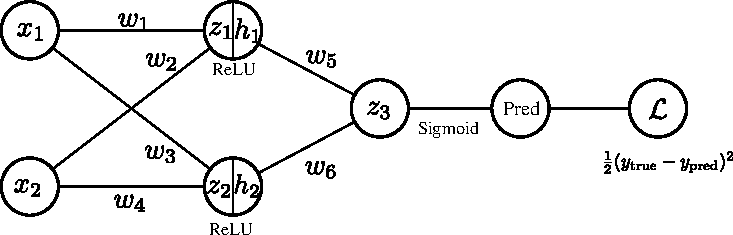
\includegraphics[scale=1.0]{./images/backprop.pdf}
\end{figure}

We have:

\begin{itemize}
	\item Inputs: $x_1, x_2$.
	\item Hidden layer: 2 neurons, each with no bias (for simplicity).  
	\item Weights $w_1, w_2, w_3, w_4, w_5, w_6$
	\item Output layer: 1 neuron, also with no bias.  
\end{itemize}

Where:
\begin{itemize}
	\item $z_1 = w_1 \, x_1 + w_2 \, x_2,\quad h_1 = \text{ReLU}(z_1)$
	\item $z_2 = w_3 \, x_1 + w_4 \, x_2,\quad h_2 = \text{ReLU}(z_2)$
	\item $z_3 = w_5 \, h_1 + w_6 \, h_2,\quad y_{\text{pred}} = \sigma(z_3)$
\end{itemize}

\begin{align*}
	\sigma(z) = \frac{1}{1 + e^{-z}}.
\end{align*}

We will train on one example $\{x=[x_1, x_2], y_\text{true}\}$.

% ---

% ## 2. Chosen Numerical Example

% - **Single training sample**:  
%   \(\displaystyle x_1 = 1.0,\quad x_2 = 0.0,\quad y_{\text{true}} = 1.0.\)
  
% - **Initial weights** (just for demonstration):  
%   \[
%     w_1 = 0.5, \quad w_2 = -0.5, \quad
%     w_3 = 0.3, \quad w_4 =  0.1, \quad
%     w_5 = 0.2, \quad w_6 = -0.1.
%   \]

Loss function: Mean Squared Error (MSE) for one sample:
  \[
    L = \frac{1}{2}\,\bigl(y_{\text{pred}} - y_{\text{true}}\bigr)^2.
  \]

We want to find the partial derivatives:

\begin{align*}
  \frac{\partial L}{\partial w_1},\;
  \frac{\partial L}{\partial w_2},\;
  \frac{\partial L}{\partial w_3},\;
  \frac{\partial L}{\partial w_4},\;
  \frac{\partial L}{\partial w_5},\;
  \frac{\partial L}{\partial w_6}.
\end{align*}


Useful Derivatives:
\begin{itemize}
	\item Derivative of the MSE loss (single sample):
	   \[
		 \frac{\partial L}{\partial y_{\text{pred}}}
		 = \bigl(y_{\text{pred}} - y_{\text{true}}\bigr).
	   \]
	\item Sigmoid derivative:
	   \[
		 \frac{d}{dz}\,\sigma(z) = \sigma(z)\,\bigl(1 - \sigma(z)\bigr).
	   \]
	   So,
	   \[
		 \frac{\partial y_{\text{pred}}}{\partial z_3} 
		 = y_{\text{pred}}\,(1 - y_{\text{pred}}).
	   \]
	\item Chain rule:  
	   \[
		 \frac{\partial L}{\partial z_3}
		 = \frac{\partial L}{\partial y_{\text{pred}}}
		   \;\times\; \frac{\partial y_{\text{pred}}}{\partial z_3}.
	   \]
\end{itemize}

The output node has:

\[
  z_3 = w_5\,h_1 + w_6\,h_2,
  \quad
  y_{\text{pred}} = \sigma(z_3).
\]

First, find \(\frac{\partial L}{\partial z_3}\):  
  \[
    \frac{\partial L}{\partial z_3}
    = (y_{\text{pred}} - y_{\text{true}}) \;\times\; 
      \bigl[y_{\text{pred}}\,(1 - y_{\text{pred}})\bigr].
  \]

Then,
  \[
    \frac{\partial L}{\partial w_5}
    = \frac{\partial L}{\partial z_3} \times \frac{\partial z_3}{\partial w_5}
    = \frac{\partial L}{\partial z_3} \times h_1.
  \]
Since \(z_3 = w_5\,h_1 + w_6\,h_2\), so \(\partial z_3/\partial w_5 = h_1\).

Each hidden neuron influences the output via \(h_1\) or \(h_2\). Let’s do them one neuron at a time.

#### 4.3.1. Hidden Neuron 1 (\(w_1, w_2\))

\[
  z_1 = w_1\,x_1 + w_2\,x_2,
  \quad
  h_1 = \sigma(z_1).
\]

To get \(\tfrac{\partial L}{\partial w_1}\), we chain through:

\[
  \frac{\partial L}{\partial w_1}
  = \frac{\partial L}{\partial z_3} 
    \,\times\, \frac{\partial z_3}{\partial h_1}
    \,\times\, \frac{\partial h_1}{\partial z_1}
    \,\times\, \frac{\partial z_1}{\partial w_1}.
\]

- We already have \(\frac{\partial L}{\partial z_3} = -0.12058.\)
- \(\frac{\partial z_3}{\partial h_1} = w_5\) (since \(z_3 = w_5\,h_1 + w_6\,h_2\)).
- \(\frac{\partial h_1}{\partial z_1} = \sigma(z_1)\bigl(1 - \sigma(z_1)\bigr) = h_1\,(1 - h_1)\).
- \(\frac{\partial z_1}{\partial w_1} = x_1\).

Numerically:

1. \(\frac{\partial z_3}{\partial h_1} = w_5 = 0.2.\)
2. \(h_1(1 - h_1) = 0.62246 \times (1 - 0.62246) = 0.62246 \times 0.37754 \approx 0.2350.\)
3. \(x_1 = 1.0.\)

So,

\[
  \frac{\partial L}{\partial w_1}
  = (-0.12058)\times(0.2)\times(0.2350)\times(1.0).
\]
Compute step by step:

- \((-0.12058)\times 0.2 = -0.024116.\)
- \((-0.024116)\times 0.2350 \approx -0.005667.\)

Thus,

\[
  \frac{\partial L}{\partial w_1} \approx -0.005667.
\]

For \(w_2\), the only difference is \(\frac{\partial z_1}{\partial w_2} = x_2\). Since \(x_2 = 0.0\) in our example, it follows immediately:

\[
  \frac{\partial L}{\partial w_2} = 0.
\]

#### 4.3.2. Hidden Neuron 2 (\(w_3, w_4\))

\[
  z_2 = w_3\,x_1 + w_4\,x_2,\quad h_2 = \sigma(z_2).
\]
By the same chain rule:

\[
  \frac{\partial L}{\partial w_3}
  = \frac{\partial L}{\partial z_3}
    \,\times\, \frac{\partial z_3}{\partial h_2}
    \,\times\, \frac{\partial h_2}{\partial z_2}
    \,\times\, \frac{\partial z_2}{\partial w_3}.
\]

- We have \(\tfrac{\partial L}{\partial z_3} = -0.12058.\)
- \(\tfrac{\partial z_3}{\partial h_2} = w_6 = -0.1.\)
- \(\tfrac{\partial h_2}{\partial z_2} = h_2 (1 - h_2) = 0.57444\times 0.42556 \approx 0.24450.\)
- \(\tfrac{\partial z_2}{\partial w_3} = x_1 = 1.0.\)

So,

\[
  \frac{\partial L}{\partial w_3}
  = (-0.12058)\times(-0.1)\times(0.24450)\times(1.0).
\]
Compute step by step:

1. \((-0.12058)\times(-0.1) = 0.012058.\)
2. \(0.012058 \times 0.24450 \approx 0.002950.\)

Hence,

\[
  \frac{\partial L}{\partial w_3} \approx 0.002950.
\]

For \(w_4\), again \(\partial z_2/\partial w_4 = x_2 = 0\), so:

\[
  \frac{\partial L}{\partial w_4} = 0.
\]

---

## 5. Weight Update

Let’s do **one step** of Gradient Descent with learning rate \(\eta = 0.1\). The update rule is:

\[
  w_i \;\leftarrow\; w_i \;-\; \eta\,\frac{\partial L}{\partial w_i}.
\]

### 5.1. Final Gradients Recap

- \(\displaystyle \frac{\partial L}{\partial w_1} \approx -0.005667\)  
- \(\displaystyle \frac{\partial L}{\partial w_2} = 0\)  
- \(\displaystyle \frac{\partial L}{\partial w_3} \approx 0.002950\)  
- \(\displaystyle \frac{\partial L}{\partial w_4} = 0\)  
- \(\displaystyle \frac{\partial L}{\partial w_5} \approx -0.07509\)  
- \(\displaystyle \frac{\partial L}{\partial w_6} \approx -0.06930\)

### 5.2. Updated Weights

1. \(\displaystyle w_1\):
   \[
     w_1 \leftarrow 0.5 - 0.1\times(-0.005667)
           = 0.5 + 0.0005667
           \approx 0.50057.
   \]

2. \(\displaystyle w_2\):
   \[
     w_2 \leftarrow -0.5 - 0.1\times 0 \;=\; -0.5.
   \]

3. \(\displaystyle w_3\):
   \[
     w_3 \leftarrow 0.3 - 0.1\times(0.002950)
           = 0.3 - 0.000295
           \approx 0.299705.
   \]

4. \(\displaystyle w_4\):
   \[
     w_4 \leftarrow 0.1 - 0.1\times 0 = 0.1.
   \]

5. \(\displaystyle w_5\):
   \[
     w_5 \leftarrow 0.2 - 0.1\times(-0.07509)
           = 0.2 + 0.007509
           \approx 0.20751.
   \]

6. \(\displaystyle w_6\):
   \[
     w_6 \leftarrow -0.1 - 0.1\times(-0.06930)
           = -0.1 + 0.00693
           \approx -0.09307.
   \]

---

## Recap

1. **Forward pass**:  
   - Calculated hidden neurons \(z_1, z_2\), then \(h_1, h_2\).  
   - Calculated output \(z_3\), then \(y_{\text{pred}}\).  
   - Computed the MSE loss \(L\).

2. **Backward pass**:  
   - Used the chain rule to find \(\tfrac{\partial L}{\partial w_i}\) for each weight.  
   - Observed how zero input (\(x_2=0\)) caused some gradients to be zero for this training example.

3. **Gradient Descent update**:  
   - Applied \(w_i \leftarrow w_i - \eta\,(\partial L/\partial w_i)\) with \(\eta=0.1\).

While we only did one training example and one update step, the principle is the same for multiple samples (you would sum or average the gradients across the batch). Larger networks just repeat the same chain-rule logic on more layers and neurons.

**That’s it!** This is the backpropagation process laid out in a small, fully traceable network with two hidden neurons. By doing the arithmetic yourself, you can see exactly how each weight nudges the output and how the gradients flow backward to update those weights.




\chapter{Divergence}
\section{KL Divergence between Two Normal Distribution}
\begin{align*}
D_\text{KL}(P||Q) & = \mathbb{E}_P\Big[\textrm{log}\frac{P}{Q}\Big]\\
\end{align*}
Consider two multivariate Gaussians in $\mathbb{R}^n$, $P_1$ and $P_2$

\begin{align*}
D_\text{KL}(P||Q) &= \int \left[ \frac{1}{2} \log\frac{|\Sigma_2|}{|\Sigma_1|} - \frac{1}{2} (x-\mu_1)^T\Sigma_1^{-1}(x-\mu_1) + \frac{1}{2} (x-\mu_2)^T\Sigma_2^{-1}(x-\mu_2) \right] \times p(x) dx \\
&= \frac{1}{2} \log\frac{|\Sigma_2|}{|\Sigma_1|} - \frac{1}{2} \text{tr} \left\{E[(x - \mu_1)(x - \mu_1)^T] \ \Sigma_1^{-1} \right\} + \frac{1}{2} E[(x - \mu_2)^T \Sigma_2^{-1} (x - \mu_2)] \\
&= \frac{1}{2} \log\frac{|\Sigma_2|}{|\Sigma_1|} - \frac{1}{2} \text{tr}\ \{I_n \} + \frac{1}{2} (\mu_1 - \mu_2)^T \Sigma_2^{-1} (\mu_1 - \mu_2) + \frac{1}{2} \text{tr} \{ \Sigma_2^{-1} \Sigma_1 \} \\
&= \frac{1}{2}\left[\log\frac{|\Sigma_2|}{|\Sigma_1|} - n + \text{tr} \{ \Sigma_2^{-1}\Sigma_1 \} + (\mu_2 - \mu_1)^T \Sigma_2^{-1}(\mu_2 - \mu_1)\right]
\end{align*}

Trace tricks:
$$x^TAx = tr[x^TAx] = tr[xx^TA]$$
$$tr[A+B] = tr[A]+tr[B]$$
$$E[(x-\mu)^T \Sigma^{-1} (x-\mu)]= tr(E[(x-\mu)(x-\mu)^T] \Sigma^{-1})$$
$$\Sigma = E[(X-\mu)(X-\mu)^T]=E[XX^T]-\mu\mu^T$$
$$E[XX^T] = \Sigma + \mu\mu^T$$

Note that the determinant of a diagonal matrix could be computed as product of its diagonal.



\section{Various Tricks}

\subsection{Spectral Normalization}

A persisting challenge in the training of GANs is the performance control of the discriminator. The derivative of discriminator could be unbounded and even incomputable, so they introduced a regularization on the derivative of discriminator called, Lipchitz continuity, which bound the gradient.

Neural network is actually a composite function. So if we make each function to satisfy the Lipchitz continuity, then we can make whole network satisfy it. Lipchitz continuity of a linear operator can be seen as 

\begin{align*}
	||f(x_1)-f(x_2)||_2 &\leq L||x_1-x_2||_2\\
	||Ax_1-Ax_2||_2 &\leq L||x_1-x_2||_2\\
	\frac{||Ax||_2}{||x||_2}&\leq L\\
	\sigma_{max}\underbrace{\sup_x \frac{||Ax||_2}{||x||_2}}_{Spectral Norm}&\leq L, \quad \textrm{Since inequaility holds for all }x
\end{align*}
, where $\sigma_{max}$ is the maximum singular value. Note that the spectral norm is from the linear algebra. We can make the matrix $A$ Lipchitz continuous by 
\begin{align*}
1 = \underbrace{\sup_x \frac{||\frac{A}{\sigma_{max}}x||_2}{||x||_2}}_{Spectral Norm}\leq L
\end{align*}


\subsection{Moving Averaging}

\subsection{Weight Averaging}

\subsection{Quality Measurements}

\section{f-Divergence}
In probability theory, an $f$-divergence is a function $D_{f}(p||q)$ that measures the difference between two probability distributions $p$ and $q$. It helps the intuition to think of the divergence as an average, weighted by the function $f$, of the odds ratio given by $p$ and $q$.

For distributions $p$ and $q$, f-divergence is defined as:
$$D_{f}(p||q) = \int_{\mathcal{X}}f\Bigg(\frac{p(x)}{q(x)}\Bigg)q(x)dx$$

\begin{itemize}
	\item KL-divergence: $f(t) = t\log t$
	\item Reversed KL-divergence: $f(t) = -\log t$
	\item Total variation: $f(t) = \frac{1}{2}|t-1|$
	$$D_{f}(p||q) = \int_{\mathcal{X}}|p(x)-q(x)|dx$$
\end{itemize}

\section{Lipchitz Continuous}
The function $f$ in the new form of Wasserstein metric is demanded to satisfy $\| f \|_L \leq K$, meaning it should be $K$-Lipschitz continuous.

A real-valued function $f: \mathbb{R} \rightarrow \mathbb{R}$ is called $K$-Lipschitz continuous if there exists a real constant $K\geq 0$ such that, for all $x_1, x_2 \in \mathbb{R}$
$$\lvert f(x_1) - f(x_2) \rvert \leq K \lvert x_1 - x_2 \rvert$$

\section{Singular Value}
All singular values can be calculated via the singular value decomposition (SVD)
$$A = U\Sigma V^T$$
, where $U$ is the left singular vectors and $V$ is the right singular vectors. However, if we just want the maximum singular value then we just need to find corresponding vectors
$$\sigma = uAv^T$$
Actually, there is a simpler way to find the maximum singular value e.g., power iteration. 



\end{appendices}
